
The construction in the previous section results in prover complexity which is quasi-linear in both the
size of the RAM and the number of operations.
Our goal in this section is to achieve prover complexity which is {\em sublinear} in the size of the RAM.
In what follows, let $N$ denote the size of the RAM (upper-case to signify it's large) and $m$ denote the number
of operations in a batch. We will use a vectors in $\F^N$ to denote the ``large'' RAMs, where index column is implicitly
assumed to be $(1,\ldots,N)$.
Let $\vec{T},\vec{T'}\in \F^N$ denote the initial and final RAM states, and let $\vec{o}$ be
a sequence of $m$ operations which updates $\vec{T}$ to $\vec{T}'$. Let $\vec{a}\in \F^m$ denote the vector
of RAM indices referenced by the operations in $\vec{o}$, i.e, $a_i$ is the index referenced by $i^{th}$ operation.
To prove the transformation of $\vec{T}$ to $\vec{T}'$ via operation sequence $\vec{o}$, we proceed as follows:
\begin{itemize}[leftmargin=2em, label=-]
    \item We isolate sub-tables $S=(\vec{a},\vec{v})$ and $S'=(\vec{a},\vec{a'})$ of $T$ and $T'$ consisting of
    rows corresponding to indices in $\vec{a}$. This requires proving $\vec{v}=\vecT[\vec{a}]$ and $\vec{v'}=
    \vecT'[\vec{a}]$, which we show using {\em committed index lookup} discussed in Section ~\ref{subsec:committed-index-lookup}.

    \item On the isolated sub-table $S$ and $S'$ of size $m$, we use the standard memory checking arguments (c.f. argument
    presented in Section \ref{sec:poly-proto-ram-app}) to prove that sequence $\vec{o}$ correctly updates $S$ to $S'$ with
    prover complexity of $\wt{O}(m)$.

    \item Finally, we show that the RAMs $T$ and $T'$ are identical outside indices in $\vec{a}$. We call them $\vec{a}$-identical
    and describe the protocol for proving the same in Section ~\ref{subsec:proximity-ram}.
\end{itemize}

\begin{figure}[htbp]
    \centering
    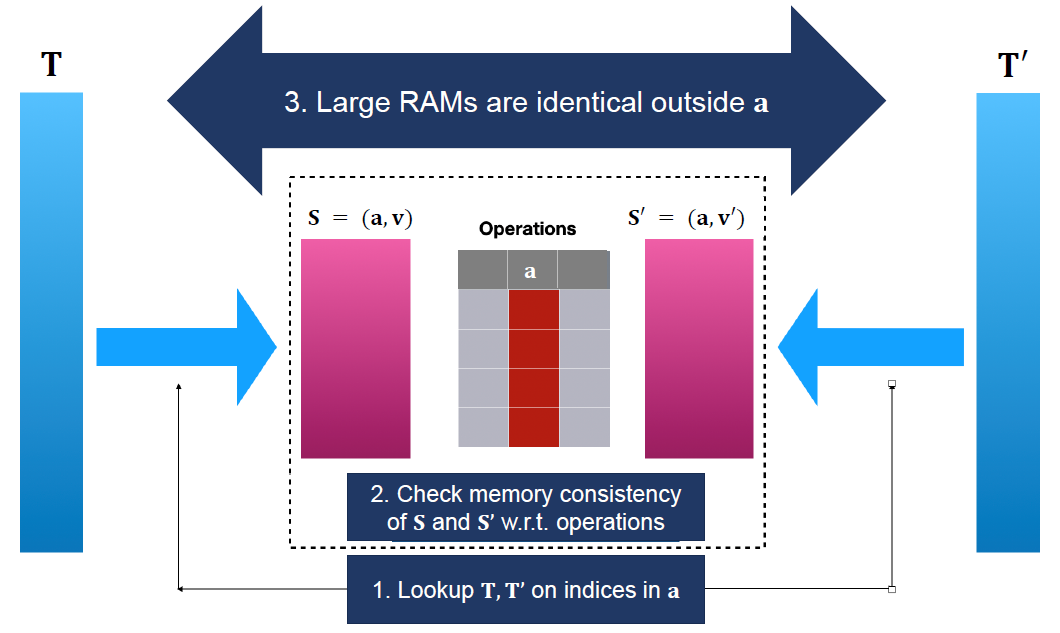
\includegraphics[width=0.4\textwidth]{RAM-Lookup}
    \caption{Illustrating different steps of sub-linear lookup protocol between large RAMs $\vecT$ and $\vecT'$.}
    \label{fig:blueprint}
\end{figure}

The blueprint for the above approach is illustrated in Figure ~\ref{fig:blueprint}.
The efficiency of the above approach relies crucially on the efficiency of committed index lookup used to
reduce the size of the RAMs for quasi-linear memory checking methods. It is tempting to use the recent lookup arguments
in ~\cite{CCS:ZBKMNS22,EPRINT:PosKat22,EPRINT:EagFioGab22} to prove the correctness of the first step with prover complexity dependent only on $m$.
However, employing them directly is difficult; their table-independent efficiency relies on
table specific expensive pre-computation, which does not help when the table is updatable. This is the problem we solve
in Section ~\ref{sec:update-protocol}, where we modify the prover algorithm for the lookup arguments to remain efficient
with access to pre-computed parameters for an ``approximate'' table.
\begin{comment} %repetition
In particular, we show that lookup protocols in
~\cite{CCS:ZBKMNS22,EPRINT:PosKat22,EPRINT:EagFioGab22} can be used to show $m$ lookups from a table $\vecT'$, given pre-computed parameters
for a table $\vecT$ with additional overhead of $O((m+\delta)\log^2 (m+\delta))$, where $\delta$ denotes the hamming distance
of tables $\vecT$ and $\vecT'$. By optimally deferring the $O(N\log N)$ re-computation till we
accumulate $\delta \approx \sqrt{mN}$ updates, we achieve an amortized prover overhead $O(\sqrt{mN})$ over the lookup protocols for non-updatable tables.
This modification described in ~\ref{sec:update-protocol} applies to all the aforementioned lookup protocols.
\end{comment}

\noindent{\bf Additional Notation}:
%Before proceeding, we introduce the subgroup $\setN=\{\xi,\ldots,\xi^N\}$ consisting of $N^{th}$ roots of unity,
%over which we encode vectors in $\F^N$ as polynomials of degree less than $N$. Let $\{\mu_i(X)\}_{i=1}^N$ be the associated
%lagrange basis polynomials over the set $\setN$. 
We introduce the set $\setV$ consisting of $m^{th}$ roots of unity
$\nu,\ldots,\nu^m$ with associated lagrange polynomials as $\{\tau_i(X)\}_{i=1}^m$. For $\vec{f}\in \F^N$, let
$\enc{f}{\setN}$ denote the polynomial encoding of $\vec{f}$ over $\setN$ given by $\sum_{i=1}^N f_i\mu_i(X)$. Similarly,
for $\vec{g}\in \F^m$, let $\enc{g}{\setV}$ denote its polynomial encoding over $\setV$ given by $\sum_{i=1}^m g_i\tau_i(X)$. 
For vectors $\vec{t}$, we sometimes use the index notation $\vec{t}[a_i]$ to denote $a_i^{th}$ element of the vector. For vectors
$\vec{t}$ and $\vec{a}$ we use the notation $\vec{t}[\,\vec{a}\,]$ to denote the vector $\vec{v}$ such that $v_i=\vec{t}[\,a_i\,]$ for all $i$.
%\chaya{above can be pruned. some of it is already in prelims.}


\subsection{Committed Index Lookup}\label{subsec:committed-index-lookup}
Let $m,N\in \N$ be fixed parameters with $m < N$ and let $\srs$ denote a $\kzg$ setup of degree $d\geq N$
over bi-linear group $(\F$, $\Gone$, $\Gtwo$, $\GT$, $e$, $\gone{1}$, $\gtwo{1}$, $[1]_t)$. Recall that the committed index
lookup relation in Definition ~\ref{defn:comm-index-lookup} involves the prover showing knowledge of vectors $\vecT\in \F^N$,
$\vec{a}\in \F^m$ and $\vec{v}\in \F^m$ corresponding to public commitments $c_T, c_a$ and $c_v$ such that they
satisfy $v_i = \vecT[\,a_i\,] = T_{a_i}$.
We present a polynomial protocol for the same, which is an adaptation of the lookup protocol from Caulk+ ~\cite{EPRINT:PosKat22}.
However, here we do not aim for zero-knowledge. Let $T(X)=\enc{t}{\setN}$, $a(X)=\enc{a}{\setV}$ and
$v(X)=\enc{v}{\setV}$ denote the polynomials encoding the vectors $\vec{t},\vec{a}$ and $\vec{v}$ respectively.
The verifier knows commitments to these polynomials at the start of the protocol.
Now $v_i = \vec{t}[a_i]$ for $i\in [m]$ is equivalent to $v(\nu^i) = T(\xi^{a(\nu^i)})$ for $i\in [m]$. To
obtain a polynomial protocol, the prover interpolates a polynomial $h(X)=\sum_{i=1}^m \xi^{a_i}\tau_i(X)$, which satisfies
$h(\nu^i)=\xi^{a(\nu^i)}$. To show that polynomial $h$ correctly ``exponentiates'' evaluations of $a(X)$, we consider the
inverting polynomial $\ell(X)=\sum_{i=1}^N i\mu_i(X)$ which behaves like ``log'' over $\setN$ by evaluating to $i$ on $\xi^i$. Now, we see
that all constraints are encoded as polynomial identities below:
\begin{equation}
    \begin{aligned}
        \ell(h(X)) &= a(X) \quad \text{mod } Z_{\setV}\\  % & \quad\text{ encodes } & \quad \forall i\in [m]:& h(\nu^i) = \xi^{a(\nu^i)}  \\
        T(h(X)) &= v(X) \quad \text{mod } Z_\setV \\ % \quad\text{ encodes } & \quad \forall i\in [m]:& v_i = \vec{t}[a_i] \\
        Z_{\setN}(h(X)) &= 0 \qquad \text{mod } Z_\setV  %&\quad\text{ encodes } & \quad \forall i \in [m]:& h(\nu^i)\in \setN
    \end{aligned}
    \label{eq:comm-index-lookup}
\end{equation}
The last polynomial identity ensures that evaluations of $h$ on $\setV$ lie in $\setN$ (the set of roots of $\vpolyN$). Since the polynomial $\ell$ is one-one
over $\setN$, the first equation implies $h(\nu^i)=\xi^{a_i}$ for all $i\in [m]$. The desired relation $v_i=T_{a_i}$ now follows from the second identity.
The above formulation involves composition with polynomials $\ell,T$ and $\vpolyN$ of degree $O(N)$, which is inefficient. We use the trick from
\cite{EPRINT:PosKat22}, where we work with low-degree restrictions of $O(N)$-degree polynomials such as $T, \ell$ over the set
$\setN_I=\{{h(\nu^i)}: i\in [m]\}=\{\xi^{a_i}:i\in I\}\subseteq \setN$, where $I=\{a_i: i\in [m]\}$. The prover
commits to the polynomials $Z_I(X)=\prod_{i\in I}(X-\xi^i)$, $h(X)$ and low degree ($<m$) restrictions $T_I, \ell_I$ of $T$ and $\ell$
on the $\setN_I$ respectively. The polynomial protocol then checks the following:
\begin{equation}
    \begin{alignedat}{3}
        T(X) - T_I(X) &= 0 \quad \text{ mod } Z_I ,&\quad& T_I(h(X)) &= v(X) \quad \text{ mod } Z_{\setV} \\
        \ell(X) - \ell_I(X) &= 0 \quad \text{ mod } Z_I ,&\quad& \ell_I(h(X)) &= a(X) \quad \text{ mod } Z_{\setV} \\
        Z_{\setN}(X) &= 0 \quad \text{ mod } Z_I ,&\quad& Z_I(h(X)) &= 0 \quad \text{ mod } Z_{\setV}
    \end{alignedat}
    \label{eq:poly-comm-index}
\end{equation}
It must be noted that the above identities imply the earlier polynomial identities in \eqref{eq:comm-index-lookup}. This is so because evaluations
of $h$ on $\setV$ are roots of $Z_I$, which implies $T_I(h(\nu^i))=T(h(\nu^i))$, $\ell_I(h(\nu^i))=\ell(h(\nu^i))$ and $\vpolyN(h(\nu^i))=0$ over $\setV$.
While the identities on the left still involve a degree $N$ polynomial, we can use the $\srs$ to check the polynomial
identity at the point $\tau$ encoded in the $\srs$. For example, we can evaluate the encoded quotient $\gtwo{Q(X)} =$
$\gtwo{\frac{(T(X) - T_I(X)}{Z_I(X)}}$ using the relation:
\begin{equation*}
    \gtwo{\frac{T(X)-T_I(X)}{Z_I(X)}} = \sum_{i\in I}\frac{1}{Z_I'(\xi^i)}\gtwo{\frac{T(X)-t_i}{X-\xi^i}}
\end{equation*}
By pre-computing the $\kzg$ proofs $W_1^i=\gtwo{\frac{T(X)-t_i}{X-\xi^i}}$ for all $i\in [N]$, the encoded quotient can be
evaluated using $O(m)$ $\Gtwo$-operations and $O(m\log^2 m)$ $\F$-operations.
The identity is then checked using a real pairing check
$$e(\gone{T(X)}-\gone{T_I(X)},\gtwo{1})=e(\gone{Z_I(X)},\gtwo{Q(X)}).$$
Similarly, we also pre-compute the encoded
quotients $W_2^i=\gtwo{\frac{\ell(X) - i}{X-\xi^i}}$ and $W_3^i=\gtwo{\frac{\vpolyN(X)}{X-\xi^i}}$ for all $i\in [N]$.
The quotients can be computed in time $O(N\log N)$ using the techniques in ~\cite{EPRINT:FeiKho23}. Using $\kzg$ commitment
scheme the polynomial relations over $Z_\setV$ can be checked in a standard manner
by having the prover send evaluation proofs for the committed polynomials at a random point chosen by the verifier.
The total prover effort incurred is $O(m^2)$ group and field operations.
Thus, we have:
\begin{lemma}\label{lem:comm-index-lookup}
Assuming $\kzg$ is extractable polynomial commitment scheme, there exists a succinct argument of knowledge for
the relation $\RLOOK$ with prover complexity of $O(m^2)$, given access to pre-computed parameters of size $O(N)$.
\end{lemma}

\subsubsection{Committed Index Lookup: Generic Transformation}\label{subsubsec:generic-transformation}
The protocol for committed index lookup using Caulk+ ~\cite{EPRINT:PosKat22} can become prohibitive for higher values of
$m$ due to the quadratic dependence on it. Here we describe a generic transformation, which realizes a committed index lookup
argument from any sub-vector argument such as ~\cite{CCS:ZBKMNS22,EPRINT:PosKat22,EPRINT:ZGKMR22,EPRINT:EagFioGab22} using a homomorphic
vector commitment scheme. We recall that $\vec{a}\in \F^m$ is called a sub-vector of $\vec{b}\in \F^n$ if each element of $\vec{a}$
also occurs in $\vec{b}$. We use $\vec{a}\leq \vec{b}$ to denote $\vec{a}$ is a sub-vector of $\vec{b}$.
The transformation follows from the observation in the following lemma:
\begin{lemma}\label{lem:generic-transformation}
Let $\vec{t}\in \F^n$ and let $\vec{a},\vec{v}\in \F^m$ for some positive integers $m,n$. Let $\vec{I}_n$ denote the vector $(1,\ldots,n)$.
Then for $\gamma\gets \F$, $\vec{a}\leq \vec{I}_n$, $\vec{v}\leq \vec{t}$ and $(\vec{v}+\gamma \vec{a})\leq (\vec{t} + \gamma \vec{I}_n)$ implies
$\vec{v}=\vec{t}[\,\vec{a}\,]$ except with probability $O(n/|\F|)$.
\end{lemma}
The proof of the Lemma appears in Section ~\ref{sec:generic-transformation-app}.
Using Lemma ~\ref{lem:generic-transformation}, allows construction of argument for proving $\vec{v}=\vec{t}[\,\vec{a}\,]$ using three instantiations
of a sub-vector argument. We require homomorphism of the commitment scheme to enable the verifier to compute commitments for $\vec{v}+\gamma \vec{a}$ and
$\vec{t} + \gamma \vec{I}_n$ for the final instantiation of sub-vector argument. In particular, we also benchmark committed index lookup
protocol using lookup argument in ~\cite{EPRINT:EagFioGab22}, which incurs prover complexity of $O(m\log m)$.
~

\subsection{Almost Identical RAM States}\label{subsec:proximity-ram}
For a vector $\vec{a}\in [N]^m$, let $\uniq{a}=\{a_i: i\in [m]\}$ denote the subset of unique values in $\vec{a}$. We call two
RAM states $\vecT, \vecT'\in \F^N$ to be $\vec{a}$-{\em identical} if $\vecT[i]=\vecT'[i]$ for all $i\not\in\uniq{a}$. As before,
let $T(X),T'(X)$ and $a(X)$ be polynomials encoding the vectors $\vecT,\vecT'$ (over $\setN$) and $\vec{a}$ (over $\setV$). Given
commitments $c_T, c_T'$ and $c_a$ polynomial protocol to prove that committed vectors $\vecT,\vecT'\in \F^N$ and $\vec{a}\in \F^m$
are such that $\vecT,\vecT'$ are $\vec{a}$-identical involves proving the relation $Z_I(X)(T(X) - T'(X)) = 0$ over $Z_\setN$ where
$I=\uniq{a}$ and $Z_I(X)=\prod_{i\in I}(X-\xi^i)$ denotes the vanishing polynomial for the set $\setN_I=\{\xi^i: i\in I\}$.
The prover commits to polynomial $Z_I$ and proves (i) $Z_I(T - T') = 0 \text{ mod } Z_\setN$ and (ii) $Z_I$ is the vanishing
polynomial of the set $\setN_I$ as defined. To prove the first relation, the prover computes the polynomial $D(X)$ as below:
\begin{align}\label{eq:poly-q}
D(X) &= \frac{(T(X)-T'(X))\cdot Z_I(X)}{Z_\setN(X)} \nonumber \\
&= \sum_{i\in I}\frac{(t_i - t_i')\mu_i(X)}{Z_\setN(X)} Z_I(X) \nonumber \\
\intertext{ Substituting, $\Delta_i=t_i-t_i'$, $\mu_i(X)=\vpolyN(X)/(\vpolyN'(\xi^i)(X-\xi^i))$ }
&=\sum_{i\in I}\frac{\Delta_i}{Z_\setN'(\xi^i)}\left(\frac{Z_I(X)}{X-\xi^i}\right) = \sum_{i\in I}\frac{\Delta_i Z_I'(\xi^i)}{Z_\setN'(\xi^i)}\kappa_i(X)
\end{align}
In the above, the summation only runs over indices in $I$, as $\Delta i = 0$ for $i\not\in I$. In the final equality, we use
$\kappa_i(X) = Z_I(X)/(Z_I'(\xi^i)(X-\xi^i))$ for $i\in I$ which we recognize as the lagrange basis polynomials for the set
$\{\xi^i: i\in I\}$. Thus, Equation \eqref{eq:poly-q} implies that $D(X)$ is at most degree $|I|-1$ polynomial, with
$D(\xi^i)=\Delta_i Z_I'(\xi^i)/\vpolyN'(\xi^i)$ for $i\in I$.
The prover can therefore interpolate $D(X)$ (in power basis)
in $O(|I|\log^2 |I|)$ $\F$-operations and compute $\gone{D(X)}$ in $O(|I|)$ $\Gone$-operations. The prover sends the
commitment $\gone{D(X)}$ to the verifier. Finally, the verifier can
check the identity $Z_I(T - T') = D\cdot Z_\setN$ by a pairing check. For this, since the tables are committed in $\Gone$, prover will need to send $\elttwo{Z_I(X)}$.

Next, the prover needs to show that $Z_I(X)$ is indeed the vanishing polynomial of $\setN_I$.
We again use the polynomial $h(X)=\sum_{i=1}^m \xi^{a_i}\tau_i(X)$ which interpolates the vector $(\xi^{a_1},\ldots,\xi^{a_m})$.
The correctness of the $h$ polynomial can be established by checking the polynomial identities in the last two rows of Equation
~\eqref{eq:poly-comm-index}. The aforementioned identities show that $Z_I(h(X)) = 0$ over $Z_\setV$ which shows that $Z_I$ vanishes over
entire vector interpolated by $h$ over $\setV$. To assert that $Z_I$ has no additional roots, the prover commits to the product polynomial
$K(X)=\prod_{i=1}^m (X - h(\nu^i))$ and the quotient polynomial $q(X)=K(X)/Z_I(X)$. The verifier checks the polynomial identities
at $\alpha$, i.e $K(\alpha)=q(\alpha)Z_I(\alpha)$ and $K(\alpha)=\prod_{i=1}^m(\alpha - h(\nu^i))$.
The former is easily accomplished
using evaluation proofs for $K,q$ and $Z_I$ at $\alpha$
For checking the latter, the prover commits to another polynomial
$u(X)$ satisfying $u(\nu^i)=\prod_{j=1}^{i-1}\big((\alpha - h(\nu^j))/(1 + \beta\tau_1(\nu^j))\big)$ for $i\in [m]$
where $\beta=K(\alpha) - 1$.
The verifier ensures the correctness of $u(X)$ by
\begin{equation}
    \begin{aligned}
        \tau_1(X)(u(X) - 1) &= 0 \text{ mod } Z_{\setV} \\
        u(\nu X)(1+\beta \tau_1(X))-u(X)(\alpha - h(X)) &= 0 \text{ mod } Z_\setV.
    \end{aligned}
    \label{eq:kh-check}
\end{equation}
We prove that the above constraints imply that $K(\alpha)=\prod_{i\in [m]}(\alpha - h(\nu^i))$.
Note that in this protocol we require commitment to the polynomial $Z_I$ in both $\Gone$ and $\Gtwo$,
and thus another pairing check is required to show that the $Z_I(X)$ committed in $\Gone$
(whose well formation is shown in the protocol as described above) is the same as the $Z_I(X)$ committed in $\Gtwo$,
used for the real pairing check.
\begin{lemma}\label{lem:kh-check}
There exists a polynomial $u(X)\in \F[X]$ satisfying the identities in Equation ~\eqref{eq:kh-check}
if and only if $K(\alpha)=1+\beta=\prod_{i\in [m]} (\alpha - h(\nu^i))$.
\end{lemma}
\begin{proof}
    Assume that the identitites hold for some polynomial $u(X)$.
    The first identity implies $u(\nu)=1$. From the second identity, we conclude that for all $i\in [m]$, we have
    $u(\nu^{i+1})=u(\nu^i)\cdot ((\alpha - h(\nu^i))/(1+\beta \tau_1(\nu^i)))$, and thus:
    $$1 = u(\nu^{m+1})/u(\nu) = \prod_{i\in [m]}\left(\frac{\alpha - h(\nu^i)}{1+\beta \tau_1(\nu^i)}\right).$$
    We observe that the product of denominators in the above equation is simply $1+\beta$ as $\tau_1(\nu^i)$
    is $0$ for all $i\neq 1$, and thus $1+\beta = \prod_{i=1}^m (\alpha - h(\nu^i))$. In the other direction,
    it is easy to check that $u(X)$ as defined for an honest prover, satisfies the identities in Equation ~\ref{eq:kh-check}.
\end{proof}

\noindent{\em Remark}: Note that we incur $O(m^2)$ cost if we show the correctness of polynomial $h$ using techniques of Section ~\ref{subsec:committed-index-lookup}.
However, we can use more $O(m\log m)$ complexity committed index lookup obtained from ~\cite{EPRINT:EagFioGab22}, which allows us to show correctness of
$h(X)$ by proving that it interpolates vector $\vec{h}$ on $\setV$ obtained as committed index lookup using vector $\vec{a}$ on the vector $\vecT_{exp}=(\xi,\xi^2,\ldots,\xi^N)$
i.e., $\vec{h}=\vecT_{exp}[\, \vec{a}\,]$.

\subsection{Batching-Efficient RAM: Combined Protocol}\label{subsec:all-together}
We put the entire protocol together now. Let $\setind$ denote the set of indices $\{1,\ldots,N\}$, and $\mathcal{I}_N$
denote the vector $(1,\ldots,N)$. We formally define the committed RAM relation for which we present an argument of
knowledge in this section.
\begin{definition}\label{defn:committed-ram}
We define the {\em committed ram} relation
$\CRAM$ to consist of tuples $((c_T, c_T', c_\op, c_a, c_w),(\vecT, \vecT',\vec{\op},\vec{a},\vec{w}))$
such that:
\begin{itemize}[leftmargin=1em]
    \item $(T,\vec{o},T')\in \LRAM{I}{N}{m}$ for $T=(\setind_N,\vecT)$, $T'=(\setind_N,\vecT')$ and $\vec{o}=(o_1,\ldots,o_m)$
    where $o_i=(\op_i, a_i, w_i)\in \RAMOp{I}$ for all $i\in [m]$.
    \item $c_T=\KZGcommit(\srs, T(X))$, $c_T'=\KZGcommit(\srs, T'(X))$, $c_\op = \KZGcommit(\srs,\op(X))$,  $c_a=\KZGcommit(\srs, a(X))$,
    $c_w = \KZGcommit(\srs, w(X))$ where polynomials $T(X), T'(X)$ encode vectors $\vecT, \vecT'$ over $\setN$, while $\op(X), a(X)$ and
    $w(X)$ encode vectors $\vec{\op}=(\op_1,\ldots,\op_m)$, $\vec{a}$ and $\vec{w}$ over $\setV$.
\end{itemize}
\end{definition}
As outlined in the blueprint, the prover first commits to ``smaller'' RAMs $S=(\vec{a},\vec{v})$ and $S'=(\vec{a},\vec{v}')$
where $\vec{v}=\vecT[\vec{a}]$ and $\vec{v}'=\vecT'[\vec{a}]$. The prover commits to $S$ and $S'$ by sending commitments
$c_v$ and $c_v'$ to $\vec{v}$ and $\vec{v}'$. Then the prover and verifier execute the committed index lookup protocol to
prove:
\begin{equation}
(c_T, c_a, c_v)\in \RLOOK\, \wedge\, (c_T', c_a, c_v')\in \RLOOK
\end{equation}
The verifier uses a random challenge $\chi\gets \F$ to reduce two instances of $\RLOOK$ to one instance
$(c_T + \chi c_T', c_a, c_v + \chi c_v')\in \RLOOK$. Then, we show that
RAMs $\vecT$ and $\vecT'$ are $\vec{a}$-identical using the protocol in Section \ref{subsec:proximity-ram}.
All that remains is to prove is that the operation sequence $\vec{o}$ is consistent with small RAMs $S$ and $S'$.
We check this using the argument in Section ~\ref{sec:poly-proto-ram}. Specifically, the prover and the verifier set
$c_S = (c_a, c_v)$, $c_S'=(c_a, c_v')$ and $c_o = (c_\op, c_a, c_w)$, and execute the argument of knowledge for
showing $(c_S, c_o, c_S')\in \CLRAM$ (see Definition ~\ref{defn:committed-ram}). We provide the complete protocol
listing in Figure ~\ref{fig:complete-listing}. The protocol in Figure ~\ref{fig:complete-listing} assumes pre-computed parameters
for the tables $T$ and $T'$. In the next section, we discuss how to efficiently maintain table-dependent parameters in the setting
requiring updates to the table.

\begin{theorem}\label{thm:committed-ram}
The protocol in Figure~\ref{fig:complete-listing} (continued in Figures~\ref{fig:complete-listing-2} and
~\ref{fig:complete-listing-3}) is a succinct argument of knowledge for the relation $\CLRAM$ in
the AGM, under the $Q$-DLOG assumption for the bilinear group $(\F,\Gone,\Gtwo,\GT,e,g_1,g_2)$.
\end{theorem}

%%% complete protocol listing %%%
\begin{figure}[t!]
    \begin{mdframed}

        \underline{Setup $(1^\secp,N,m, \vecT, \vecT')$}:
        \begin{itemize}[leftmargin=1em]
            \item $\srs = (\{\gone{\tau^i}\}_{i=0}^N, \{\gtwo{\tau^i}\}_{i=0}^N)$ for $\tau\gets \F$.
            \item $W_2^i=\gtwo{(\ell(X) - i)/(X-\xi^i)}$, $i\in [N]$(needed by prover)
            \item $W_3^i=\gtwo{\vpolyN(X)/(X-\xi^i)}$, $i\in [N]$(needed by prover)
            \item $\gone{\ell(X)}, \gone{\vpolyN(X)}, \gtwo{\vpolyN(X)}$(known by both)
        \end{itemize}

        \underline{Precompute $(\vecT, \vecT')$}:
        \begin{itemize}[leftmargin=1em]
            \item $W_1^i=\gtwo{(T(X)-T(\xi^i))/(X-\xi^i)}$, $i\in [N]$,
            \item ${W_1^i}'=\gtwo{(T'(X) - T'(\xi^i))/(X-\xi^i)}$, $i\in [N]$.
        \end{itemize}

        {\bf Common Input}: $\srs$, $c_T, c_T', c_\op, c_a, c_w\in \Gone$.\\
        {\bf Prover's Input}: Vectors $\vecT,\vecT',\vec{\op},\vec{a},\vec{w}$ and their encoding polynomials.\\

        {\bf Round 1}: Commit to sub RAMs.
        \begin{enumerate}[leftmargin=1em, label=\arabic*.]
            \item $\prover$ computes $\vec{v}=\vecT[\,\vec{a}\,]$, $\vec{v}'=\vecT'[\,\vec{a}\,]$ and the encoding
            polynomials $v(X)$ and $v'(X)$.
            \item $\prover$ sends $c_v = \gone{v(X)}$, $c_v'=\gone{v'(X)}$.
            \item $\verifier$ sends $\chi\gets \F$.
        \end{enumerate}

        {\bf Round 2}: Execute committed index lookup.
        \begin{enumerate}[leftmargin=1em, label=\arabic*.]
            \item $\prover$ and $\verifier$ compute $C_T=c_T + \chi c_T'$, $C_V=c_v + \chi c_v'$.
            \item $\prover$ computes $P(X) = T(X) + \chi T'(X)$, $V(X)=v(X) + \chi v'(X)$.
            \item $\prover$ computes $I=\{a_i: i\in [m]\}$, $\setN_I=\{\xi^i: i\in I\}$.
            \item $\prover$ computes polynomials:
            \begin{itemize}[leftmargin=1em, label=-]
                \item Vanishing polynomial $Z_I(X)$ of $\setN_I$.
                \item Polynomial $h(X)=\sum_{i\in [m]}\xi^{a_i}\tau_i(X)$.
                \item Restrictions $P_I(X),\ell_I(X)$ of $P(X),\ell(X)$ on set $I$.
                \item $K(X)=\prod_{i\in [m]}(X-\xi^{a_i})$, $q(X)=K(X)/Z_I(X)$
                \item $D(X)= \sum_{i\in I}\frac{\Delta_i Z_I'(\xi^i)}{Z_\setN'(\xi^i)}\kappa_i(X)$ by interpolation as described in section 5.2
            \end{itemize}

            \item $\prover$ sends $c_p = \gone{P_I(X)}$, $c_z=\gone{Z_I(X)}$, $c_{z2}=\gtwo{Z_I(X)}$, $c_h=\gone{h(X)}$, $c_l = \gone{\ell_I(X)}$,
            $c_k = \gone{K(X)}$, $c_q = \gone{q(X)}$, $c_d=\gone{D(X)}$
            \item $\verifier$ sends $\gamma\gets \F$.
        \end{enumerate}

        {\bf Round 3}: Prover send aggregated quotients.
        \begin{enumerate}[leftmargin=1em, label=\arabic*.]
            \item $\prover$ computes $g(X)=P_I(X) + \gamma \ell_I(X) + \gamma^2 Z_I(X)$.
            \item $\prover$ computes $Q(X) = (g(h(X)) - v(X) -\gamma a(X))/Z_\setV(X)$.
            \item $\prover$ computes: $W = \sum_{i\in [m]} \frac{1}{Z_I'(\xi^i)} (W_1^i + \chi {W_1^i}' + \gamma W_2^i + \gamma^2 W_3^i)$.
            \item $\prover$ sends $W\in \Gtwo$, $c_Q=\gone{Q(X)}$.
            \item $\verifier$ computes $c_g = c_p + \gamma c_l + \gamma^2 c_z$, $C_G = C_T + \gamma\gone{\ell(X)}+\gamma^2\gone{\vpolyN(X)}$.
            \item $\verifier$ checks: $e(C_G - c_g, \gtwo{1})=e(c_z, W)$.
            \item $\verifier$ checks: $e(c_T-c_{T'}, c_{z2})=e(c_d, \gtwo{\vpolyN(X)})$
            \item $\verifier$ checks: $e(c_z, [1]_2)=e([1]_1, c_{z2})$
            \item $\verifier$ sends $\alpha\gets \F$.
        \end{enumerate}

        Continued in Figure ~\ref{fig:complete-listing-2}
    \end{mdframed}
    \caption{Batching-Efficient RAM Protocol}
    \label{fig:complete-listing}
\end{figure}






\section{Fast Lookups from Approximate Pre-Processing}\label{sec:update-protocol}


Recall that our lookup protocol in section 5.1 involves certain precomputations by the prover namely $W_1^i, W_2^i, W_3^i$. $W_2^i$ and $W_3^i$ do not depend on the table. However, $W_1^i$ depends on the lookup table and their values will change even if the table changes by a small amount. It is expensive to recompute all the $W_1^i$ for every small change in the table and this will affect the efficiency of our lookup protocol in the long run.\\\\
In this section, we show how to achieve efficient lookups even when the table is changing frequently, as long as the cumulative change in the table is small. \\
In particular, we show how the prover can compute $[Q(X)]_2=\gtwo{\frac{T(X)-T_I(X)}{Z_I(X)}}$ without computing all the $W_1^i$(thus minimizing the overhead).\\
The overhead(as long as the table doesn't change too much) will be much lower than the time needed for the lookup and so is very practical.

\subsection{The idea: Base + Cache approach}

The idea is that we do not compute $W_1^i$ after each change of the table. Instead, this expensive computation will be done periodically for all $i \in [N]$ after say $s \in \mathbb{Z}$ batches.
Let current table $\vecT$ can be represented as $\vecTbase + \vecTcache$ where the vector
$\vecTbase$ denotes the base table (with respect to which $W_1^i$ was last computed for all $i \in [N]$) and the vector $\vecTcache$ corresponds to the changes
that have happened to the base table since the last rebasing (rebasing denotes computation of all $W_1^i$)\\\\
Thus, there is an \textbf{online} phase which happens after every batch (which includes computation of $[Q(X)]_2$ among other things) and an \textbf{offline} phase which consists of the rebasing(this is all prover computations) \\\\




\noindent{\bf Offline Phase}: This computation is executed once after every $s$ rounds. Here, the prover updates the base vector $\vecTbase$ with the changes in the cache vector
$\vecTcache$ by setting $\vecTbase := \vecTbase + \vecTcache$ and simultaneously clears the cache vector by setting
$\vecTcache = 0$.\\
It computes the commitment of $T_b$ as well\\
It also re-computes the $\mathsf{KZG}$ opening proofs $[W_1^i(x)]_2$ for $i\in [N]$ where
$W_1^i(X) = (\Tbasepoly{X} - t_i)/(X-\xi^i)$. Here, $t_i=\Tbasepoly{\xi^i}$ are the coordinates
of the updated base vector $\vecTbase$.\\
As mentioned in section 5.1 this can be done in $O(N\log N)$ group and field operations.\\\\
\noindent{\bf Online Phase}:
The online phase happens for every batch because the purpose of this phase is to ensure that all the things needed for the current execution of the lookup protocol are available. We show how the prover computes the next table $T'$ from the current table $T$ and the new Cache vector from the old cache vector (by an inductive argument this suffices)
\begin{enumerate}[leftmargin=1em]
    \item Prover has the $T$ for the current round and the commitment $[T(x)]_1$ as well(because these are just the $T'$, $[T'(x)]_1$ of the last round)
    \item The $\vecTcache$ and $\vecTcache(X)$ is also updated to the start of the current round (contains information till previous round:$\vecT=\vecTbase+\vecTcache$)
    \item The prover updates the cache using the current batch: $\vec{T'}_{\mathsf{ch}}[i] = \vec{T}_{\mathsf{ch}}[i] + \Delta_i$ for $i\in I$ in $O(m)$ $\F$ operations
    \item Here $\Delta_i$ for all $i \in I$ is the change that will happen to $\vecT$ \textbf{during the current round}
    \item Prover computes the commitment to the new cache polynomial:
    $$[\vec{T'}_{\mathsf{ch}}(x)]_1=[\vec{T}_{\mathsf{ch}}(x)]_1+\sum_{i\in I}\Delta_i[\mu_i(x)]_1$$ in
    $O(m)$ $\Gone$ operations.
    \item Prover also gets ${T}'$ as ${T'}[i]=T_b[i]+ \vec{T'_{\text{ch}}}[i]$ using the $T_b$ and the latest cache
    \item Prover computes the commitment to the new table $\vecT'$: $[T'(x)]_1=[\Tbasepoly{x}]_1+[\vec{T'}_{\mathsf{ch}}(x)]_2$

    \item In addition, the other things (apart from $[Q(x)]_2$) needed for the current round of the lookup protocol are also computed by the prover as described in the lookup protocol in section 5.1 as it is just naive computation



\end{enumerate}

\subsection{Computation of $[Q(X)]_2$}
Clearly, it suffices to efficiently compute $[Q(x)]_2$ where $[Q(x)]_2=\gtwo{\frac{T(x)-T_I(x)}{Z_I(x)}}$. We have the information of $[\Tbasepoly{x}-\Tbasepoly{\xi^i}/(x-\xi^i)]_2$. For this, we have the following lemma:


\begin{lemma}\label{lem:approx-setup}
Let $N,\xi$ be as defined previously. Suppose we are given
$\kzg$ proofs $\{W_i\}_{i=1}^N$ with $W_i=\gtwo{\Tbasepoly{X} - \Tbasepoly{\xi^i}/(X-\xi^i)}$ and where
$\Tbasepoly{X}=\enc{T_{\mathsf{b}}}{\setN}$ encodes a vector $\vecTbase\in \F^N$.
Let $I \subset [N]$.
Then,
there exists an algorithm to compute $\kzg$ multi-opening proof
$[Q(X)]_2=\gtwo{(T(x) - T_I(x)/Z_I(x)}$ for encoding $T(X)=\enc{T}{\setN}$ of vector $\vecT\in \F^N$ using $O((\delta + |I|) \log^2 (\delta + |I|))$ $\F$-operations and $O(\delta + |I|)$ $\Gtwo$-operations.
Here, $\delta$ denotes the hamming distance
between vectors $\vecTbase$ and $\vecT$.
\end{lemma}

\begin{proof}
    We know that $\vecT=\vecTbase+\vecTcache$ and that $T(X)=\Tbasepoly{X}+\Tcachepoly{X}$\\

    Let $K \subset [N]$ be a set which contains $I$ and all those indices $j$ for which $\vecTcache[j] \neq 0$. For these $j$, let $\vecTcache[j]=\Delta t_j$. Then $\Tcachepoly{X}=\sum_{j\in K}\Delta t_j\mu_j(X)$.\\\\
    By definition of $K$, $|K|\leq \delta +|I|$. So, we need to bound $\Gtwo$ operations by $O(|K|)$ and field operations by $O(|K| \log^2|K|)$\\
    First of all note that:
    \begin{align}\label{eq:Q2-upd}
    Q_2(X) &= \sum_{i\in \setind}\frac{1}{z_I'(\xi^i)}\left(\frac{\Tbasepoly{X} - \Tbasepoly{\xi^i}}{X-\xi^i}\right)
    + \sum_{i\in \setind}\frac{1}{z_I'(\xi^i)}\left(\frac{\Tcachepoly{X} - \Tcachepoly{\xi^i}}{X-\xi^i}\right)
    \end{align}

    From the above we can write $\elttwo{Q_2(x)}=\gtwo{\Qbasepoly{x}}+\gtwo{\Qcachepoly{x}}$ where
    \begin{gather*}
        \Qbasepoly{X}=\sum_{i\in \setind}(z_I'(\xi^i))^{-1} (\Tbasepoly{X}-\Tbasepoly{\xi^i})/(X-\xi^i) \\
        \Qcachepoly{X}=\sum_{i\in \setind}(z_I'(\xi^i))^{-1} (\Tcachepoly{X}-\Tcachepoly{\xi^i})/(X-\xi^i)
    \end{gather*}
    We can compute
    $\elttwo{\Qbasepoly{x}}$ from the pre-computed KZG openings of $\Tbasepoly(X)$ at points $\xi^i,i\in I$ using $O(|I|)$ group operations and
    $O(|I|\log^2 |I|)$ field operations(as is done in Caulk/Caulk+).\\\\

    \textbf{Thus, it suffices to describe the computation for $\elttwo{\Qcachepoly{x}}$. }\\
    Using
    $\Tcachepoly{X}=\sum_{j\in K}\Delta t_j\mu_j(X)$ and defining constants $c_i=(1/z_I'(\xi^i))$ for $i\in I$,
    we write $\Qcachepoly{X}$ as:
    \begin{align*}
        \Qcachepoly{X} &= \sum_{i\in \setind} c_i\sum_{j\in K} \Delta t_j\frac{\mu_j(X)-\mu_j(\xi^i)}{X-\xi^i} \\
        &= \sum_{i\in \setind} c_i\Delta t_i\frac{\mu_i(X) - 1}{X-\xi^i} + \sum_{i\in \setind}\sum_{j\in K\setminus\{i\}}c_i\Delta t_j\frac{\mu_j(X)}{X-\xi^i}
    \end{align*}
    Now, we can write $\elttwo{\Qcachepoly{x}}=\elttwo{\Qcachepolyone{x}} + \elttwo{\Qcachepolytwo{x}}$ where:
    \begin{gather*}
        \Qcachepolyone{X}=\sum_{i\in \setind}c_i\Delta t_i\frac{\mu_i(X)-1}{X-\xi^i} \\
        \Qcachepolytwo{X}=\sum_{i\in \setind}\sum_{j\in K\setminus \{i\}} c_i\Delta t_j\frac{\mu_j(X)}{X-\xi^i}
    \end{gather*}

    The term $\elttwo{\Qcachepolyone{x}}$ can be computed using $O(I)$ group operations by pre-computing the
    \textsf{KZG} openings of polynomials $\mu_i(X)$ at $\xi^i$ for $i\in [N]$. That is by precomputing $[\frac{\mu_i(X)-1}{X-\xi^i}]_2$. This requires just $N$ more precomputations and can be done along with the other precomputations which are done in the lookup protocol\\

    \textbf{Thus, it suffices to describe the computation for $\Qcachepolytwo{X}$}:
    \begin{align}\label{eq:Qcachepoly2}
    \Qcachepolytwo{X} &= \sum_{i\in \setind}c_i\sum_{j\in K\setminus \{i\}} \Delta t_j\mu_j(X)/(X-\xi^i) \nonumber \\
    &= \sum_{i\in\setind}c_i\sum_{j\in K\setminus \{i\}}\frac{\Delta t_j}{Z_{\nroots}'(\xi^j)} \frac{Z_{\nroots}(X)}{(X-\xi^i)(X-\xi^j)} \nonumber \\
    \intertext{This used definition of $\mu_j(X)$}
    \intertext{ Now, using $Z_\nroots'(\xi^j)=N\xi^{-j}$ and partial fraction decomposition}
    &\Qcachepolytwo{X}= N^{-1}\sum_{i\in\setind}c_i\sum_{j\in K\setminus \{i\}}\frac{\xi^j\Delta t_j}{\xi^i-\xi^j}
    \left(\frac{Z_\nroots(X)}{X-\xi^i} - \frac{Z_\nroots(X)}{X-\xi^j}\right) \nonumber \\
    &\Qcachepolytwo{X}= N^{-1}\sum_{i\in\setind}\left(c_i\cdot \sum_{j\in K\setminus \{i\}} \frac{\xi^j\Delta t_j}{\xi^i-\xi^j}\right)\frac{Z_\nroots(X)}{X-\xi^i} \nonumber \\
    &\qquad + \sum_{j\in K}\left(\xi^j\Delta t_j\cdot \sum_{i\in \setind\setminus \{j\}}\frac{c_i}{\xi^j-\xi^i}\right)\frac{Z_{\nroots}(X)}{X-\xi^j}
    \end{align}
    In this last equality, the first term is just the first term of the distributive property in finite fields.\\
    The second term is just the second term of the distributive property in finite fields except that the order of the sums is reversed. This follows from the following fact \\

    \begin{fact}
        $\sum_{i \in I} \sum_{j \in K \setminus \{i\}} f(i,j)=\sum_{j \in K} \sum_{i \in I \setminus \{j\}} f(i,j) $
    \end{fact}

    In the above equation \eqref{eq:Qcachepoly2}, let us define:
    \begin{gather*}
        a_i = \sum_{j\in K\setminus \{i\}}\frac{\xi^j\Delta t_j}{\xi^i-\xi^j}, \text{ for } i\in \setind \\
        b_j=  \sum_{i\in \setind\setminus \{j\}}\frac{c_i}{\xi^j - \xi^i}, \text{ for } j\in K \\
        W_3^i(X) = \frac{Z_\nroots(X)}{X-\xi^i}, \text{ for } i\in [N]
    \end{gather*}


    Then, we have:
    \begin{equation}\label{eq:Qcachepoly2commit}
    \elttwo{\Qcachepolytwo{x}} = N^{-1}\left(\sum_{i\in\setind}c_ia_i\elttwo{W_3^i(x)} + \sum_{j\in K}\xi^j \Delta t_j b_j \elttwo{W_3^j(x)}\right)
    \end{equation}

    $c_i$ for all $i \in \setind$ are determined easily by evaluating $Z_{\setind}'(X)$ on $H_{\setind}$ and $[W_3^i(X)]_2$ for all $i \in [N]$ have been computed in the lookup protocol

    So, given $\{a_i\}_{i\in I}, \{b_j\}_{j\in K}$, $\elttwo{\Qcachepolytwo{x}}$ can be computed in $O(|\setind|+|K|)\, \Gtwo$ operations.\\
    But $|\setind|+|K|<2|K|$. So, $\Gtwo$ operations are $O(|K|)$ as required.\\\\

    It remains to bound the number of field operations needed to compute the scalar multipliers $a_i, i \in \setind$ and $b_j, j \in K$. \\

    Let us consider $a_i$ first:\\
    Note that:

    $$ a_i = -\sum_{j\in K\setminus \{i\}}\Delta t_j + \xi^i\sum_{j\in K\setminus \{i\}}\frac{\Delta t_j}{\xi^i-\xi^j} $$
    This is because:
    $$a_i+\sum_{j\in K\setminus \{i\}}\Delta t_j= \sum_{j \in K \setminus \{i\}}\frac{\xi^j\Delta t_j}{\xi^i-\xi^j}+\Delta t_j$$
    $$=\sum_{j \in K \setminus \{i\}}\frac{\xi^i\Delta t_j}{\xi^i-\xi^j} = \xi^i\sum_{j\in K\setminus \{i\}}\frac{\Delta t_j}{\xi^i-\xi^j}$$
    Now, define $\Delta T=\sum_{j\in K}\Delta t_j$\\

    Here computing $\Delta T$ is a one time computation (per batch). It can be computed from the knowledge of $T_{\text{ch}}$ in the online phase.
    We have:
    $$ a_i = -\Delta T + \Delta t_i + \xi^i\sum_{j\in K\setminus\{i\}}\frac{\Delta t_j}{\xi^i-\xi^j} $$
    Suppose we get $\sum_{j\in K\setminus\{i\}}\frac{\Delta t_j}{\xi^i-\xi_j}$ for all $i \in I$ efficiently. Then $a_i$ for all $i \in I$ can be obtained in $O(|I|)$ field operations. \\
    \textbf{Thus, to get $a_i$ for all $i \in I$ it suffices to describe the computation of $e_i=\sum_{j\in K\setminus\{i\}}\frac{\Delta t_j}{\xi^i-\xi^j}$ for all $i \in I$}\\\\
    Our requirement is now to bound the number of field operations for $e_i$ and for $b_j$. For this, we invoke the following lemma with the proof in the appendix.

    \begin{lemma}\label{lem:sum computation}
    Let $e_i$ for all $i \in \setind$ and $b_j$ for all $j \in K$ be as described above.
    Then, $e_i$ for all $i \in I$ and $b_j$ for all $j \in K$ can be computed in $O(|K|\log^2|K|)\, \mathbb{F}$ operations
    \end{lemma}

    From the lemma \ref{lem:sum computation}, we have shown that the field operations needed to get $e_i$ and $b_j$ and thus $\elttwo{\Qcachepolytwo{x}}$ is $O(|K|\log^2|K|)$. \\

    This completes the proof of Lemma \ref{lem:approx-setup}.
\end{proof}

\subsection{Amortized Analysis of the update protocol}
Recall that we were able to get $[Q(X)]_2$ in $O(|K|)$ group operations and $O(|K|\log^2|K|)$ field operations. \\
For concrete analysis, let $s$ be the period after which the rebasing takes place. Also, the lookup happens at maximum of $m$ indices during a single batch. Thus, $|I|\leq m$.\\
This gives an upper bound on $\delta$, that is $ms$ and an upper bound on $K$, that is $ms+m=m(s+1)$.\\

Clearly $O(K)=O(ms)$ and $O(|K|\log^2|K|)=O(ms \log^2(ms))$ so group operations are $O(ms)$ and field operations are $O(ms\log^2(ms))$ \\

Moreover, after every $s$ batches, the rebasing(offline phase) is done which we know takes $O(N\log N)$ group and field operations.\\

So, the amortized number of operations for the offline and online phase in total is:
$O(ms \log^2(ms)+\frac{N\log N}{s})$ $\mathbb{F}$ operations and $O(ms +\frac{N\log N}{s})$ $\Gtwo$ operations\\

The value of $s$ which minimizes the group operations is $\sqrt{\frac{N}{m}}$. For this value of $s$:\\
\textbf{The amortized group operations needed are $\tilde{O}(\sqrt{mN})$}\\
\textbf{The amortized field operations needed are also $\tilde{O}(\sqrt{mN})$}\\
Here $\tilde{O}$ denotes that the polylog factors have been neglected\\\\














